\section{Elektronik}
\label{sec:elektronik}

\textit{Silisloth} ist aufgeteilt in einen Last- und Steuerstromkreis. Jeder der Stromkreise wird von einem eigenen Akku gespeist. Damit wird sichergestellt, dass beim Anlaufen von Komponenten mit hohem Stromverbrauch (DC-Motor, Schrittmotor) die Spannung am Raspi oder Arduino nicht zusammenbricht, was einen Neustart zur Folge hätte. Jedoch ist es wichtig die beiden Akkus auf dieselbe gemeinsame Masse (Potential null) zu bringen um ungewollte Ausgleichsströme zu verhindern. Realisiert wird dies mit einer einfachen $0.25mm^2$ Kupferverbindung zwischen den beiden Minuspolen der Akkus. \imgrefplain{fig:blockschaltbild} zeigt das Blockschaltbild mit den beiden Stromkreisen.

\subsection{Steuerstromkreis}

Der Steuerstromkreis beinhaltet die Intelligenz von \textit{Silisloth}. Spannungsquelle ist ein Lithium-Polymer-Akku ($3.7V$/$3000 mAh$). Die $3.7V$ werden über einen Step-Up-Converter von Adafruit auf $5.2V$ gebracht, welcher auch das Laden des Akkus über das Netzgerät ermöglicht. Über den Converter wird der Raspi mit Strom versorgt, welcher dann über eine USB-Schnittstelle gleichzeitig den Arduino speist. Der Raspi ist sozusagen das Gehirn von \textit{Silisloth}: er empfängt Signale von aussen, verarbeitet diese und leitet dann die nötigen Befehle oder Informationen an den Arduino oder an die App weiter. Direkt am Raspi angeschlossen über ein Flachbandkabel ist die Raspi-Kamera, welche für die Zielfelderkennung verwendet wird. Des Weiteren führt ein einfacher Taster auch direkt auf die Eingangspins des Raspis. Dieser ist zuvorderst an der Laufkatze angebracht und erzeugt ein Signal sobald der Endpfosten berührt wird, was zum sofortigen Stoppen des Antriebsmotors führt.
Über ein selbst hergestelltes PCB (Printed Circuit Board, \imgrefplain{fig:schaltung}) werden die beiden Ultraschallsensoren vom Typ HC-SR04 am Raspi angeschlossen. Diese messen zu jeder Zeit den Abstand vom Boden und zum Endpfosten. Das PCB beinhaltet lediglich vier Widerstände, welche benötigt werden um die Sensoren korrekt anzusteuern. Es erleichtert aber auch das Anschließen der Sensoren und spart Pins am Raspi. Wie bereits erwähnt wurde das Board in einfachster Art und Weise selbst hergestellt. Auf einer vorgefertigten Loch-Platte wurden die Widerstände und Anschlussklemmen aufgelötet und mit isolierten Trafo-Drähten verbunden.

\begin{figure}
    \centering
    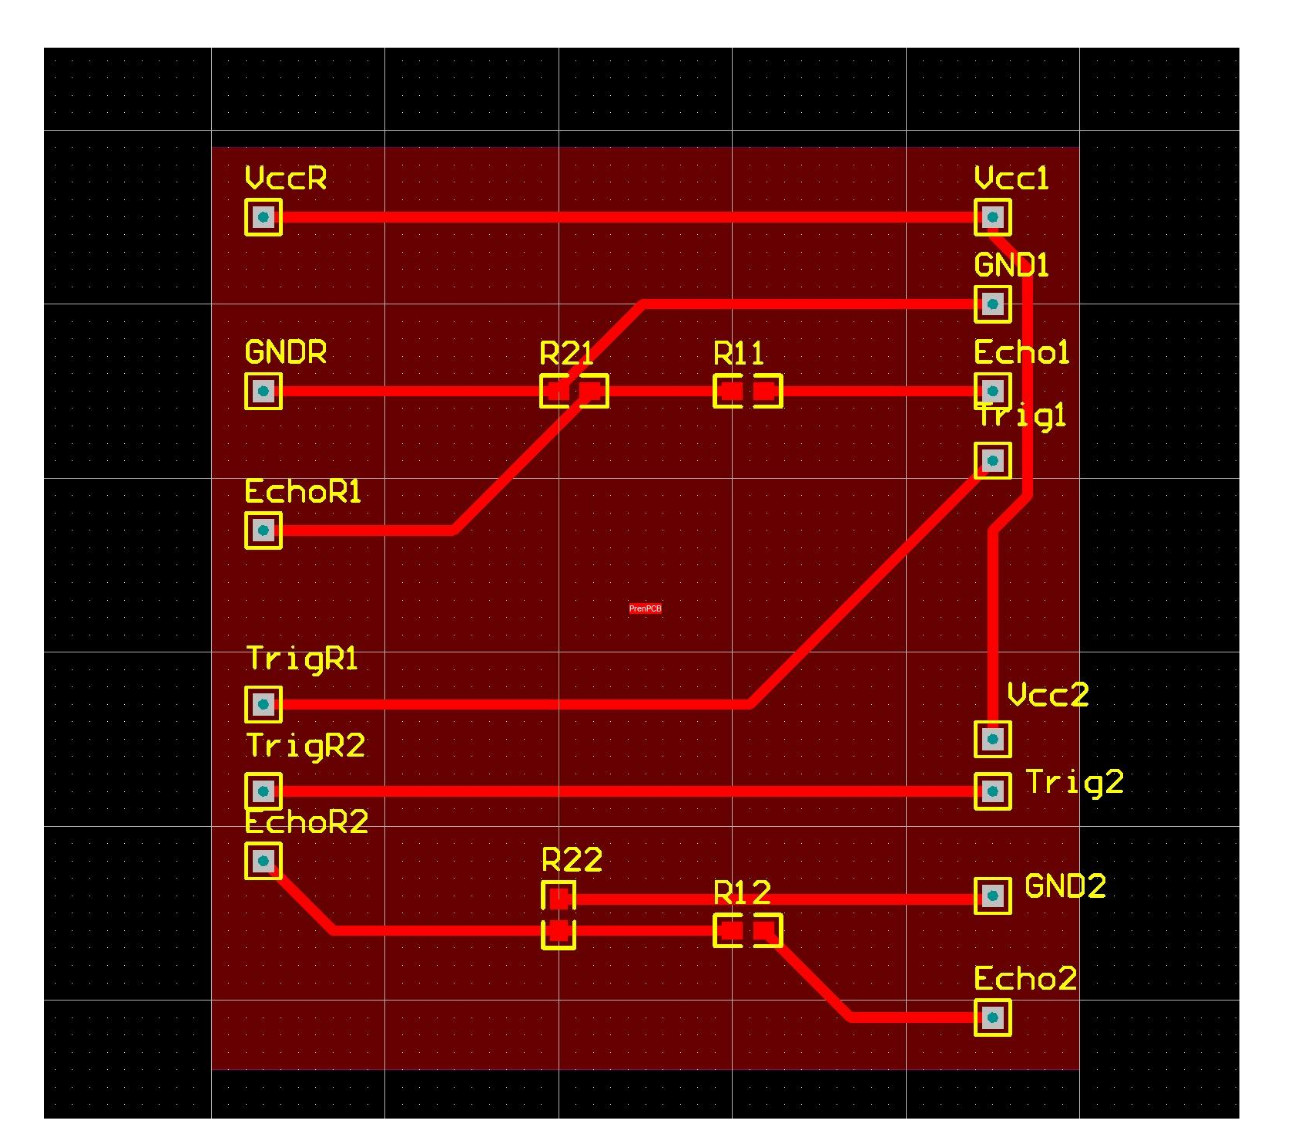
\includegraphics[width=0.5\textwidth]{pics/schaltung.jpg}
    \caption{Printed Circuit Board für die Ultraschallsensoren, die am Raspi angeschlossen sind}
    \label{fig:schaltung}
\end{figure}

\subsection{Laststromkreis}

Ein Lithium-Polymer Akku ($14.8V$/$1300mAh$) bildet die Grundlage für den Laststromkreis. Dieser besteht aus vier Zellen. Die Spannung der einzelnen Zellen darf nicht unter ca. $3.3V$ fallen, ansonsten kann der Akku nicht mehr geladen werden und wird somit unbrauchbar. Um dies zu verhindern kommt ein Spannungsüberwacher zum Einsatz, welcher am Ladeanschluss des Akkus eingesteckt wird und permanent die Zellspannungen überprüft. Gerät die Spannung einer Zelle in den kritischen Bereich, wechselt die jeweilige LED von grün auf rot.
Die $14.8V$ vom Akku sind noch ein wenig zu hoch für die übrigen Komponenten und werden deshalb über einen Step-Down-Converter auf exakt $12V$ gebracht. Mit diesen $12V$ wird das Adafruit Motor Shield v2 gespeist, welches einfach auf der Arduino aufgesteckt wird. Direkt am Motor Shield angeschlossen ist der $12V$ DC Getriebemotor Igarashi TYP 33G-50, welcher die Laufkatze antreibt, und der $12V$ bipolar Schrittmotor von SparkFun Electronics, welcher die Greifeinheit rauf und runter lässt.
In der Greifeinheit befinden sich zwei $12V$-Luftpumpen und das Magnetventil. Diese Komponenten werden über ein Spiralkabel mit Strom versorgt. Damit der Silikongreifer aufgepumpt werden kann, muss der Luftauslass des Magnetventils geschlossen sein. Dies geschieht, sobald eine Spannung von $12V$ am Ventil anliegt. Wird die Spannung unterbrochen, öffnet sich der Luftauslass und der Greifer löst sich. Um eine hohe Spannung von $12V$ mit dem Arduino zu schalten, kommt ein $5V$-Relais zum Einsatz. Dieses wird als Öffner angeschlossen, d.h. im Ruhezustand ist der Stromkreislauf zum Magnetventil geschlossen, was bedeutet, dass dieses dicht macht. Wird nun vom Arduino über den $5V$-Ausgang das Relais angesteuert, zieht dieses und unterbricht somit den Stromkreis zum Magnetventil, was bedeutet, dass der Greifer die Last loslässt. Die beiden Luftpumpen werden direkt am Motor Shield angeschlossen.

\begin{figure}
    \centering
    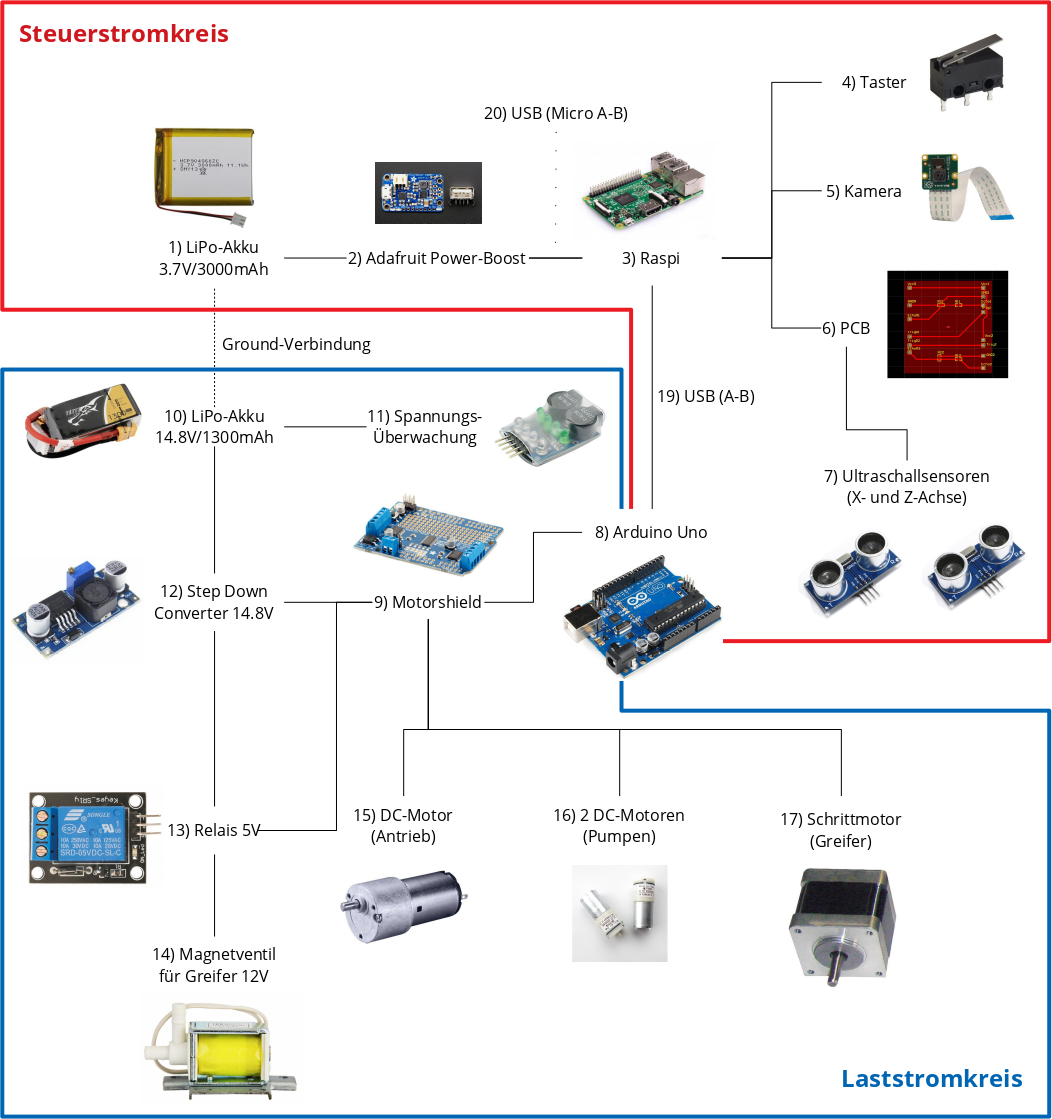
\includegraphics[width=\textwidth]{graphs/blockschaltbild.png}
    \caption{Das Blockschaltbild der Elektronik-Komponenten, aufgeteilt in einen Steuerstromkreis (rot) und einen Laststromkreis (blau). Der Arduino ist das Verbindungsglied zwischen diesen beiden Stromkreisen.}
    \label{fig:blockschaltbild}
\end{figure}

\subsection{Elektronikkomponenten}

Im Folgenden werden sämtliche verbauten Elektronikkomponenten aufgelistet. Die Nummerierung der Liste stimmt mit derjenigen auf dem Blockschaltbild (\imgrefplain{fig:blockschaltbild}) überein.

Gegenüber PREN 1 sind einige neue Komponenten dazugekommen. Da für diese in der Dokumentation zu PREN 1 \cite[S. 50]{pren1} eine Quellenangabe fehlt, ist diese bei den betreffenden Komponenten -- Arduino, Motor Shield, LiPo-Akku für Laststromkreis, Spannungsüberwacher, Step-Down-Converter, Relaismodul und Magnetventil -- hier entsprechend angefügt.

\begin{enumerate}
    \item Lithium-Polymer Akku $3.7V$/$3000mAh$ HCP90486ZC
    \item Adafruit USB PowerBoost/Charger 1A-1000C
    \item Entwicklerboard Raspberry Pi 3 Model B
    \item Taster $30V$ DC/$2A$ DC 
    \item Raspberry Pi Camera Module v2
    \item PCB (Printed Circuit Board)
    \item Ultraschallsensor HC-SR04 ($2\times$)
    \item Mikrocontroller Arduino Uno \cite{arduino}
    \item Adafruit Motor Shield v2 \cite{motorshield}
    \item RC-Akku Tattu Lithium-Polymer $1300mAh$, $14.8V$ 45C 4S1P \cite{akku}
    \item Spannungsüberwacher LiPo-Summer Pichler \cite{spannungsueberwachung}
    \item LM2596 S DC-DC Adjustable Step Down Buck Converter \cite{stepdownconverter}
    \item Relaismodul HP-ARL-5V $5V$ \cite{relais}
    \item $12V$ DC-2-Position 3-Wege elektrisches Magnetventil \cite{magnetventil}
    \item Getriebemotor $12V$ Igarashi TYP 33G-50
    \item DC5V-12V RF-370 Mini Motor Luftpumpe ($2\times$)
    \item Bipolar Stepper Motor 200 Step $0.33A$ $12V$ DC
    \item Spiralkabel $188mm/500mm$ $4\times0.12mm^2$ zwischen Kontrollbox und Greifeinheit
    \item USB 2.0 (A-B) Verbindungskabel zwischen Raspberry Pi und Arduino
    \item USB A auf Micro USB B Ladekabel für das Raspberry Pi
\end{enumerate}
